\documentclass[10pt,a4paper]{article}
\usepackage[a4paper,margin=0.75cm]{geometry}
\usepackage[utf8]{inputenc}
\usepackage[T1]{fontenc}
\usepackage{titlesec}
\usepackage{enumitem}
\usepackage[hidelinks]{hyperref}
\usepackage{fancyhdr}
\usepackage{multicol}
\usepackage{xcolor}
\usepackage{graphicx}

\definecolor{accentTitle}{HTML}{0E6E55}
\definecolor{accentText}{HTML}{0E6E55}
\definecolor{accentLine}{HTML}{A16F0B}
\definecolor{muted}{HTML}{666666}

\pagestyle{fancy}\fancyhf{}
\renewcommand{\headrulewidth}{0pt}
\renewcommand{\footrulewidth}{0pt}

\hypersetup{pdfauthor={Oualid Hmoudou},pdftitle={CV - Oualid Hmoudou},pdfsubject={Curriculum Vitae}}

\titleformat{\section}{\vspace{-4pt}\color{accentText}\raggedright\large\bfseries}{}{0em}{}[\color{accentLine}\titlerule]
\newenvironment{resume_list}{\vspace{-2pt}\begin{itemize}[itemsep=0.3pt,parsep=0pt,topsep=0.3pt,leftmargin=18pt]}{\end{itemize}\vspace{-2pt}}
\setlist[itemize]{label=\textbullet}
\newcommand{\heading}[2]{{\raggedright\noindent\textbf{#2} \quad \textbf{#1}\\}}

\setlength{\parskip}{0.5pt}
\raggedbottom\raggedright\urlstyle{same}

\begin{document}
\vspace*{-10pt}

% ── Header ──────────────────────────────────────────────────────────────────
\noindent
\begin{minipage}[t]{0.22\textwidth}\vspace{6pt}
  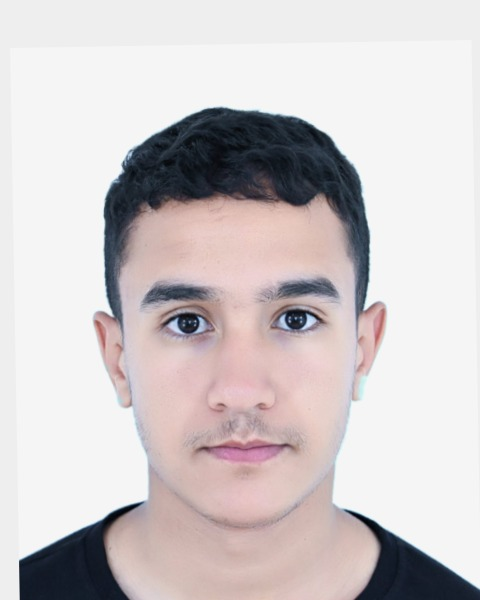
\includegraphics[width=2.5cm,height=3.3cm,keepaspectratio]{myphoto.jpeg}
\end{minipage}\hfill
\begin{minipage}[t]{0.76\textwidth}
  \begin{center}
    {\Huge\color{accentTitle} OUALID HMOUDOU}\\[4pt]
    {\color{accentLine}\hrule}\vspace{3pt}
    {\small
      +33\,6\,20\,24\,42\,27 \quad|\quad
      \href{mailto:oualidhmoudou@gmail.com}{oualidhmoudou@gmail.com} \quad|\quad
      Amiens, France \quad|\quad Permis B
    }\\[2pt]
    {\small
      \textbf{Portfolio : }\href{https://oualidhmoudou.github.io}{\color{accentText}\underline{oualidhmoudou.github.io}}
      \quad|\quad
      \href{https://linkedin.com/in/oualid-hmoudou-16880a225}{\color{accentText}\underline{LinkedIn}}
    }\\[2pt]
    {\color{accentLine}\hrule}
  \end{center}
\end{minipage}
\vspace{1pt}\centering\small\color{muted}
Étudiant Master MIAGE (M1) --- Profil hybride \textbf{Développement \textbullet{} Data/BI \textbullet{} Gestion de projet} --- Alternance dès septembre 2026\par
\vspace{3pt}\raggedright

% ── Profil ──────────────────────────────────────────────────────────────────
\section{Profil}
Étudiant en Master MIAGE à l'UPJV d'Amiens, à la croisée du \textbf{développement logiciel}, de la \textbf{Business Intelligence} et de la \textbf{gestion de projet}. Je conçois des applications fullstack de bout en bout (API REST, modélisation de bases de données), j'industrialise des tableaux de bord décisionnels (Power BI, DAX) et je pilote des projets en méthode Agile. Rigueur, qualité du code et sens du collectif --- forgés notamment par mon engagement à la Croix-Rouge Française.

% ── Compétences ─────────────────────────────────────────────────────────────
\section{Compétences techniques}
\begin{multicols}{2}
\begin{itemize}[itemsep=0.3pt,leftmargin=18pt]
  \item \textbf{Langages} : Java, C\#/.NET, PHP, Python, JavaScript, SQL
  \item \textbf{Frameworks web} : Symfony, Laravel, Vue.js, React, ASP.NET, API REST
  \item \textbf{Data \& BI} : Power BI (DAX, Power Query), SQL, Python/ML, modélisation
  \item \textbf{Bases de données} : MySQL, PostgreSQL, Oracle, SQL Server
  \item \textbf{DevOps \& outils} : Git/GitLab, GitHub Actions, Docker, Linux
  \item \textbf{Gestion de projet} : Agile/Scrum, Jira, MS Project, reporting/KPIs
  \item \textbf{Architecture \& qualité} : Clean Architecture, SOLID, design patterns, tests, revue de code
  \item \textbf{Power Platform} : Power Automate, SharePoint, Teams, Excel avancé
\end{itemize}
\end{multicols}

% ── Expériences ─────────────────────────────────────────────────────────────
\section{Expériences professionnelles}

\heading{EPSF, Amiens \textbf{--} Stage Analyste BI (Direction des Contrôles)}{Depuis juin 2026}
\begin{resume_list}
  \item Industrialisation de tableaux de bord de contrôle ferroviaire sous \textbf{Power BI} (mesures \textbf{DAX} complexes) ; automatisation et standardisation des reportings.
\end{resume_list}

\heading{Teatch, Paris \textbf{--} Stage Product Engineer (Développement Fullstack)}{Avr. -- Juin 2026}
\begin{resume_list}
  \item Refonte complète d'une plateforme web (front \& back) : conception des composants, design d'\textbf{API REST}, modélisation de la base de données.
  \item Intégration de fonctionnalités d'\textbf{IA} pour automatiser des processus métier ; qualité assurée par Git, tests unitaires, revue de code et déploiement.
\end{resume_list}

\heading{ORMVAH, Marrakech \textbf{--} Développeur Web \& Assistant Chef de Projet}{Avr. -- Juin 2023}
\begin{resume_list}
  \item Application web de gestion développée sous \textbf{Laravel} ; conception et optimisation du schéma \textbf{MySQL} (vues, procédures stockées).
  \item Recette, déploiement, formation des utilisateurs finaux et documentation technique.
\end{resume_list}

\heading{NJT Group \textbf{--} Développeur Web (Stage)}{Juin -- Août 2022}
\begin{resume_list}
  \item Application de gestion des formations développée from scratch (\textbf{PHP}, \textbf{MySQL}) avec tableaux de bord de suivi de l'activité.
\end{resume_list}

% ── Formation ───────────────────────────────────────────────────────────────
\section{Formations}
\begin{resume_list}
  \item \textbf{2025 -- En cours} \quad \textbf{Master MIAGE} (M1) -- Université de Picardie Jules Verne, Amiens
  \item \textbf{2023 -- 2025} \quad \textbf{Licence Informatique} -- Université de Picardie Jules Verne, Amiens
  \item \textbf{2021 -- 2023} \quad \textbf{DUT Génie Informatique} -- EST Essaouira, Maroc
\end{resume_list}

% ── Projets ─────────────────────────────────────────────────────────────────
\section{Projets significatifs}
\begin{resume_list}
  \item \textbf{Plateforme de Billetterie en ligne} (C\#/.NET 8, Vue.js 3, API REST, MySQL) --- application fullstack en équipe Agile/Scrum, API documentée (Swagger), pipeline CI/CD GitHub Actions.
  \item \textbf{Automatisation \& Reporting} (Power Platform) --- digitalisation d'un processus métier, tableaux de bord Power BI (modélisation, mesures DAX).
  \item \textit{Autres projets (Java \& design patterns, IA Q-learning, Clean Architecture…) détaillés sur le \href{https://oualidhmoudou.github.io}{\color{accentText}\underline{portfolio}}.}
\end{resume_list}

% ── Langues & Engagement ────────────────────────────────────────────────────
\vspace{1pt}
\begin{minipage}[t]{0.48\textwidth}
\section{Langues}
\begin{resume_list}
  \item \textbf{Français} : C1 \quad \textbf{Anglais} : C1
  \item \textbf{Arabe} : natif \quad \textbf{Espagnol} : A1
\end{resume_list}
\end{minipage}\hfill
\begin{minipage}[t]{0.48\textwidth}
\section{Engagement}
\begin{resume_list}
  \item \textbf{Croix-Rouge Française} -- Équipier Secouriste (depuis mars 2024)
\end{resume_list}
\end{minipage}

\end{document}
